\documentclass{report}
\usepackage[utf8]{inputenc}
\usepackage{graphicx}
\usepackage{url}
\usepackage{hyperref}
\usepackage{amsmath}

% \title{Sentiment Analysis - Analyzing sentiment of articles on fuel prices}
% \author{
%   Nehal Naeem Haji, 
%   Taha Munawar, 
%   Sabahatullah Shaikh, 
%   Turab Hussain Usmani
% }
% \date{}

\title{{\huge \textbf{Data Structures II \\CS 201}} \\ 

\vspace*{5mm}
{\LARGE \textbf{Final Project Report}}

\vspace*{5mm}
{\Large \textbf{Sentiment Analysis - Analyzing sentiment of articles on fuel prices using Natural Language Processing}}\\
\vspace*{3mm}
{\Large \textbf{Instructor: Faisal Alvi}}}

\author{Nehal Naeem Haji\\Taha Munawar\\Sabahatullah Shaikh\\Turab Hussain Usmani} 
\date{01 May 2024}

\begin{document}
\maketitle

\tableofcontents
\newpage

\chapter{Abstract}
\section{Context}
Fluctuations in petrol prices have a significant impact on the economy and daily lives of people. Media coverage and public sentiment surrounding petrol price changes can influence consumer behavior, policy decisions, and market dynamics. Understanding the sentiment expressed in news articles about petrol prices can provide valuable insights into public opinion and potential reactions to price fluctuations.

\section{Aim}
The primary aim of this project was to perform sentiment analysis on a collection of news articles related to petrol prices. By analyzing the sentiment expressed in these articles, we sought to gauge the overall tone and sentiment towards petrol price changes, as well as identify any patterns or trends in the sentiment over time or across different sources.

\section{Data Structures used}
The nature of this project was such that there wasn't much use of data structures. The most notable one, however, was the use of a Pandas DataFrame to store the data obtained from the sentiment analysis tools and the human readings. The data was then plotted on a graph using the Matplotlib library.

\chapter{Overview}
\section{Methods}
Our project approached the analysis with the following three different
techniques:
\begin{enumerate}
    \item \textbf{Pre-existing Sentiment Analysis Website:} : We utilized a pre-existing,
          off-the-shelf sentiment analysis tool to analyze the sentiment expressed
          in the articles. This tool leverages natural language processing
          techniques and machine learning models trained on large datasets to
          classify text as positive, negative, or neutral sentiment. These tools were
          the following websites that we found from google:
          \begin{itemize}
              \item \href{https://monkeylearn.com/sentiment-analysis-online/}{https://monkeylearn.com/sentiment-analysis-online/}
              \item \href{          https://text2data.com/Demo
                    }{          https://text2data.com/Demo
                    }
          \end{itemize}
    \item \textbf{Human Readings:} We also employed human readings of the articles. Our team members carefully read through selected articles and manually
          assigned sentiment scores based on their interpretation of the tone and
          sentiment expressed in the text. This approach provided a human validated benchmark for evaluating the performance of the automated
          sentiment analysis methods.
    \item \textbf{Custom Sentiment Analysis Program:}  We developed our own custom
          sentiment analysis program tailored specifically for the task of analyzing
          news articles about petrol prices. We first took datasets from the internet,
          which were lexicons in the English language. Each word within the set
          vocabulary was given a polarity score. The program would take a url for
          the web article, then extract the text content from the web article,
          tokenize the words, then loop through them and determine whether the
          words existed in our dataset, and calculate the polarity score
          accordingly. The dataset we used was a combined form of two pre-existing datasets on Kaggle, titled afinn.csv and bing.csv on the GitHub
          repository. A problem that we encountered was that the afinn dataset
          was too small, so we derived a formula that would combine values from
          each dataset to calculate the polarity score of the given word. Formula:
          \begin{equation}
              \text{Word score} = \frac{4 \cdot (\text{afinn score}) + \text{bing score}}{5}
          \end{equation}
          Then, the individual scores
          of all the words were added to obtain the score of an article. The code
          can be found in the main.py, also found on the \href{https://github.com/NehalNN10/TNTStrike/}{GitHub repository}.
\end{enumerate}
After utilizing these techniques, we plotted the results obtained from each
method, along with a change in fuel prices, on a graph.

\chapter{Aftermath}
\section{Results}
The graphs obtained are as follows:
\begin{itemize}
    \item Pre-existing Sentiment Analysis Website
          \\
          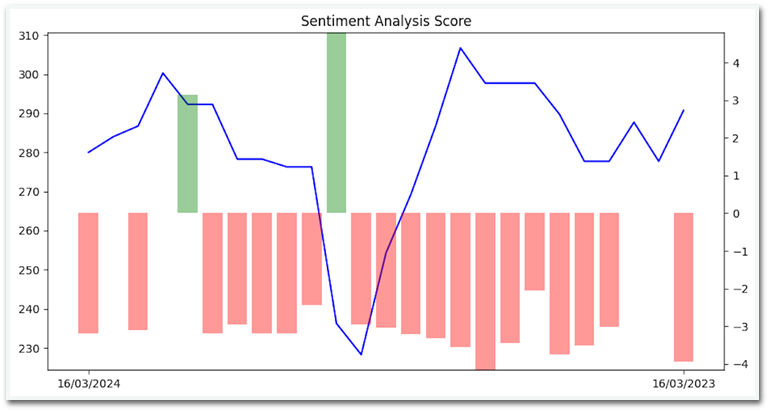
\includegraphics{images/web_analysis.png}
          \newpage
    \item Human Readings
          \\
          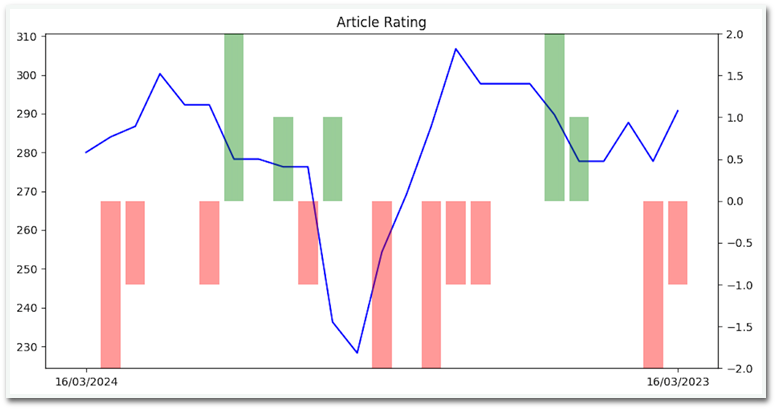
\includegraphics{images/human_readings.png}
    \item Custom Sentiment-Analysis Program
          \\
          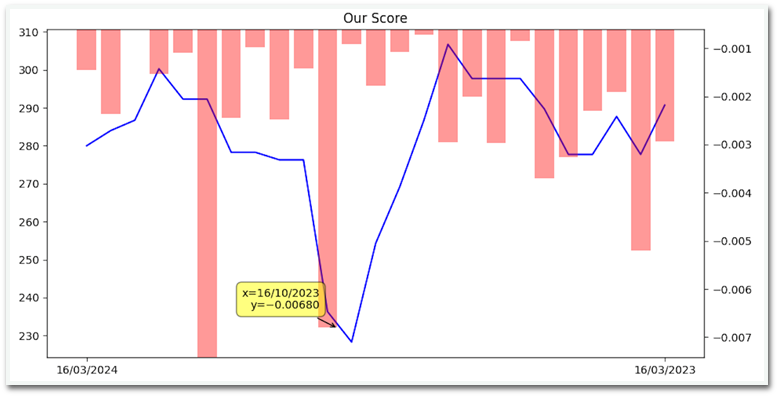
\includegraphics{images/our_program.png}
\end{itemize}

In all the graphs attached above, the blue line represents the change in fuel
prices, where as the bars showcase the polarity rating. A red bar indicates a
negative rating, while a green one indicates a positive rating. The height of
the bar determines how negative/positive an article was relative to each
other. The left hand y-axis depicts fuel price in PKR, and the right hand y-axis depicts the polarity rating. The x-axis represents the date of the article.

\section{Limitations}
As we can see from the graphs above, the pre existing sentiment analysis
and the human readings had somewhat similar scores to each other, while
our own program was negatively skewed. We believe this is because of our
“naive” approach, in which we take words literally, as they are on face value,
while not accounting for things like figures of speech, sarcasm, etc. We also
do not account for the context the word is used in. A very good example of
this is from the news article published on \href{https://www.dawn.com/news/1798239/fuel-prices-slashed-by-up-to-rs14
}{16th Dec, 2023}, in which the
headline uses the word “slashed”. Now, literally speaking, this is a negative
sounding word. However, in the context of petrol prices and the article itself,
it actually symbolizes that the government has reduced the price of petrol.
Obviously, a human reader and a complex sentiment analysis program would
be able to pick up on this, but our program was unable to do so.
\\\\
Additionally, we only used a small dataset of 25 articles, all from the same source. Dawn is a reputable news source, which might explain their use of moderate language. However, this does not represent the entire population of news articles, and thus, our results may not be generalizable to all news articles about petrol prices.
\\\\
Furthermore, petrol prices, although a very important aspect in a country's economy, is not the most politically debated of topics. This means that the articles we analyzed were not as polarized as they could have been. This could have led to a more negative bias in our results, as the articles were more neutral in tone.

\section{Conclusion and Future Work}
With all that being said, this project was a good learning experience, as it
exposed us to the domain of Natural Language Processing and could
potentially help us in future courses related to AI/ML. Based on the results we obtained, we can conclude that negative bias is present in the articles, although to a lesser degree than perhaps other news outlet articles.

\section{Work division}
\begin{itemize}
    \item Nehal Naeem Haji: Custom Sentiment Analysis Program
    \item Taha Munawar: Human Readings and Report Writing
    \item Sabahatullah Shaikh: Human Readings, Collecting Links and Presentation
    \item Turab Hussain Usmani: Pre-existing Sentiment Analysis Website
\end{itemize}

\section{Acknowledgements}
We would like to acknowledge Professor Faisal Alvi for his guidance and support throughout the project. Indeed, this project was his idea, and it opened the doors to the interesting field of Natural Language Processing. We would also like to thank our team members for their hard work and dedication to the project.

\section{Github Repository}
The code for this project can be found \href{https://github.com/NehalNN10/TNTStrike/}{here}.

\end{document}
